%% implemen.tex
%% ==============================
\chapter{Implementierung}
\label{ch:Implementierung}
Dieses Kapitel befasst sich mit der Implementierung der Algorithmen des vorherigen Kapitels. Zuerst werden jeweils die Ein- und Ausgaben der verschiedenen Nodes, deren Nutzen und Funktionsweise erklärt. 
Danach werden die einzelnen Schritte der Implementierung des NodeDialogs und NodeModels erläutert. Falls eine Implementierung eines Views vorhanden ist, wird auch dieser präsentiert.
%% ==============================
\section{Preference Creator Node}
\label{ch:Implementierung:sec:prefCreatorNode}
%% ==============================
\begin{figure}[H]
	\centering
	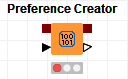
\includegraphics{prefCreatorLogo.png}
	\caption{Preference Creator Node}
	\label{img:prefCreatorLogo}
\end{figure} 

In Figur \ref{img:prefCreatorLogo} ist der Preference Creator Node zu sehen. Dieser nimmt als Eingabe eine Datenbankverbindung, in KNIME DatabasePortObject genannt, und einen BufferedDataTable an. Das DatabasePortObject enthält den Typ der Datenbankverbindung, einen SQL Query und die entsprechende Verbindung mit Datenbank URL und JDBC Treiber. Zusätzlich enthält das Objekt auch einen Benutzernamen und das dazugehörige Passwort, falls dies für die Datenbank Authentifizierung notwendig ist. Mit Hilfe des Querys und der Verbindung können Datensätze abgerufen und für den Algorithmus verwendet werden. 
In Abbildung \ref{img:prefCreatorDBConnection} ist einer dieser Objekte mit allen eingegeben Daten zu sehen, wohingegen Abbildung \ref{img:prefCreatorDataTable} einem Teil der Datensätzen des BufferedDataTables entspricht. Dieser BufferedDataTable wird für den NodeDialog benötigt, um alle Dimensionen dieser Tabelle in einer Auswahlbox anzuzeigen, da im NodeDialog die Datensätze nicht mit der Datenbankverbindung abgerufen werden können. Somit ist es notwendig, dass mit dem Query des DatabasePortObjects ein identischer BufferedDataTable entsteht, da sonst mit falschen Daten weitergearbeitet wird. Deshalb wird vor der Ausführung des Nodes geprüft, ob beide BufferedDataTables identisch sind. Falls dieser Test fehlschlägt, kann der Node nicht ausgeführt werden und dem Benutzer wird eine Fehlermeldung ausgegeben.

\begin{figure}[H]
	\centering
	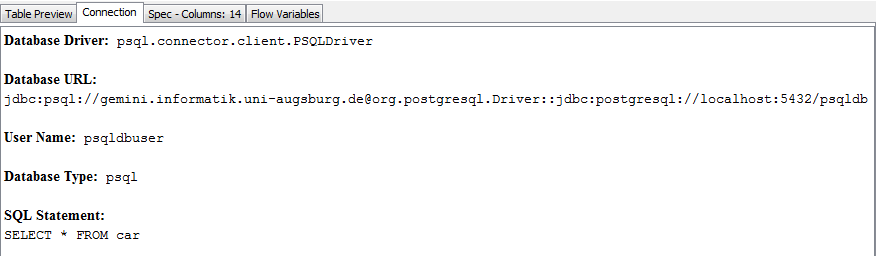
\includegraphics[width=\textwidth]{prefCreatorDBConnection.png}
	\caption{DataBaseConnection Inport des PreferenceCreator Nodes}
	\label{img:prefCreatorDBConnection}
\end{figure}

\begin{figure}[H]
	\centering
	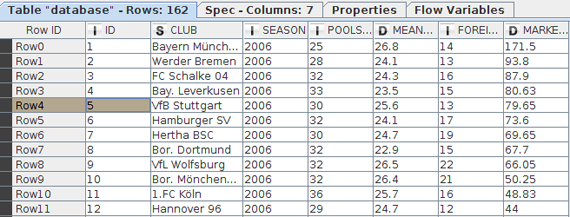
\includegraphics[width=\textwidth]{prefCreatorDataTable.png}
	\caption{BufferedDataTable Inport des PreferenceCreator Nodes}
	\label{img:prefCreatorDataTable}
\end{figure}

Bei der Ausführung des Nodes werden zwei SQL Queries erzeugt. Der Score Query und der Preference Query. Der Score Query bewertet jeden Datensatz anhand der Präferenzen, die im NodeDialog vom Benutzer eingegeben werden. Die Scores entsprechen dabei den Werten, die ein Datensatz für die Scoring Funktionen der einzelnen Basispräferenzen annimmt und drückt somit aus wie gut der Datensatz die Präferenz erfüllt. Umso niedriger der Score, desto besser erfüllt der Datensatz die Präferenz. Die einzelnen Scoring Funktionen der Basispräferenz werden später in diesem Abschnitt vorgestellt.
Im Gegensatz dazu entspricht der Preference Query einem Preference SQL Query (siehe Kapitel \ref{ch:Forschungsstand:sec:prefSQL}), welcher auf den selben Präferenzen basiert. 

Einer der Ausgaben des Nodes entspricht dem selben DataBasePortObject, welcher als Eingabe in den Node kommt. Diese Ausgabe wird von nachfolgenden Nodes benutzt, um sich mit der Datenbank zu verbinden, um dadurch auf die originalen Daten zugreifen zu können. Die meisten nachfolgende Nodes benutzen sowohl den Score Query als auch den ursprünglichen Query, der als  Zusatzinformation für das DatabasePortObject enthalten ist. Der Grund dafür ist, dass die meisten Nodes dieser Arbeit sowohl die bewerteten Datensätze, die durch den Score Query entstehen, als auch den Originaldatensatz benötigen. Um beides zu ermöglichen, werden der Score Query, der Preference Query und weitere Informationen, die später noch genannt werden, als versteckte Eingaben an folgende Nodes weitergegeben. Nachfolgende Nodes sind hierbei alle Nodes, die im vorhergehenden Datenfluss einen Preference Creator Node besitzen. Diese müssen nicht zwingend direkte Nachfolger des Preference Creator Nodes sein, sondern können auch Enkelkinder sein.

Der Preference Query wird bisher nur von dem Preference SQL Extract (siehe Abschnitt \ref{ch:Implementierung:sec:prefSQLExtract}) und dem Preference SQL Node (siehe Abschnitt \ref{ch:Implementierung:sec:prefSQL}) benutzt. 

Die zweite Ausgabe stellt die Scoretabelle da, einen BufferedDataTable der durch eine Abfrage des Score Queries an die Datenbankverbindung entsteht. Diese Ausgabe ist ein optionaler BufferedDataTable, da er nur als zusätzliche Information dient und nicht als Eingabe für folgende Nodes benötigt wird. Nachfolger können die Scoretabelle mit dem Score Query und der Datenbankverbindung selber erstellen.

\begin{figure}[H]
	\centering
	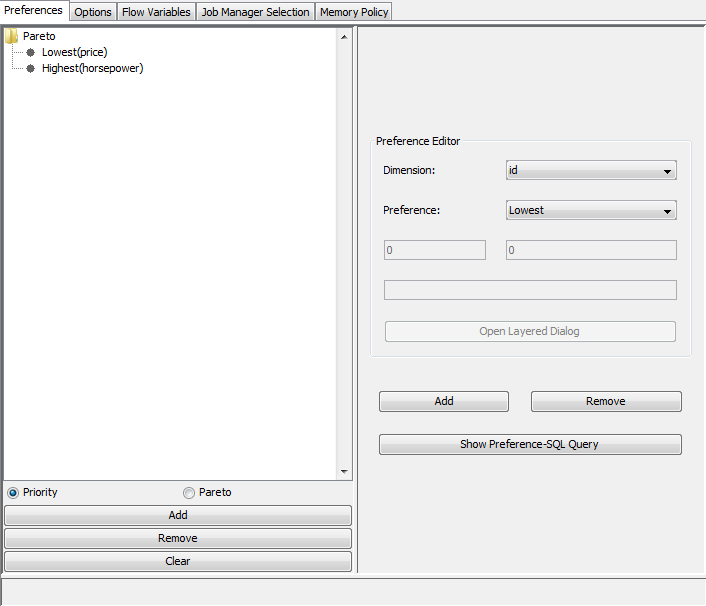
\includegraphics[width=\textwidth]{prefCreatorNodeDialog.png}
	\caption{PreferenceEditor, in dem der User seine Präferenzen einstellen kann}
	\label{img:prefCreatorNodeDialog}
\end{figure}

Für die Implementierung des NodeDialogs wurde eine eigene GUI erstellt und keine vorgegebenen Komponenten von KNIME benutzt. 
Im NodeDialog (Abbildung \ref{img:prefCreatorNodeDialog}) ist auf der linken Seite eine Baumdarstellung zu sehen. Dort können neue Prioritäts oder Pareto Knoten mit dem 'Add' Button hinzugefügt werden. Dabei kann ein Prioritätsknoten nur zu einem leeren Baum oder zu einem Paretoknoten hinzugefügt werden und umgekehrt. Weiterhin können diese Knoten einzeln mit dem 'Remove' Button oder gemeinsam mit dem 'Clear' Button entfernt werden. Mit den beiden Optionen 'Priority' und 'Pareto' kann entschieden werden, welche Knoten gerade bearbeitet werden sollen. Dies führt dazu, dass nur Prioritätsknoten hinzugefügt oder entfernt werden können, falls die entsprechende Option ausgewählt ist und vice versa.

Auf der rechten Seite kann der User durch das Selektieren eines Prioritäts oder Pareto Knotens eine Präferenz zu dem selektierten Knoten hinzufügen. Der User hat für die Erstellung einer Präferenz zwei Auswahlboxen. Eine ist für die Auswahl der Dimensionen, die den Spaltennamen des BufferedDataTables gleichen, zuständig. Die andere Box dagegen ermöglicht die Auswahl der Präferenzen für die ausgewählte Dimension. Folgende Präferenzen, deren Prinzip in Kapitel \ref{ch:Grundlagen:sec:präferenzen} genauer erklärt wurden, stehen zur Auswahl: LOWEST, HIGHEST, AROUND, BETWEEN, BOOLEAN und LAYERED. Für die AROUND, BETWEEN und BOOLEAN Präferenzen gibt es Eingabefelder für die Werte, die für diese Präferenzen benötigt werden. Diese Eingabefelder sind je nachdem, was für eine dieser Präferenzen gerade ausgewählt ist, aktiviert oder deaktiviert. Zu beachten ist, dass Dimensionen mit nicht-numerischen Werten nur mit einer LAYERED Präferenz priorisiert werden können. 
Zusätzlich zu allen vorliegenden Dimensionen gibt es eine \enquote{CustomDimension}. Diese Dimension kann der User in einem der Eingabefelder selber erstellen. Es können beispielsweise Dimensionen geteilt werden, falls ein bestimmter Prozentsatz präferiert werden soll. Dies ist vor allem im Sport sinnvoll, da dadurch gelungene Torschüsse in Vergleich zu Torschussversuchen gesetzt werden können. Es können aber auch boolische Präferenzen erstellt werden wie zum Beispiel 'price < 16000'. Der User hat damit freie Auswahl seine eigenen Dimensionen zu erstellen und diese zu präferieren. Die \enquote{CustomDimension} erlaubt alle Präferenzen außer der LAYERED Präferenz, da keine Werte vorhanden sind, da diese erst bei der Abfrage des Queries entstehen. Sie ist auch die einzige Dimension, welche die BOOLEAN Präferenz, erlaubt. 

Für die LAYERED Präferenz kann der User den LayeredDialog öffnen. Das Öffnen dieses Dialogs ermöglicht den User in einem separatem Fenster die Werte der ausgewählten Dimension nach Wichtigkeit zu sortieren.
Auf der linken Seite des LayeredDialogs kann der User positive Layer oder negative Layer hinzufügen und entfernen. Welche Layer hinzugefügt oder entfernt werden, wird durch die Option 'Negative Layers' bestimmt. Auf der rechten Seite kann der User die ausgewählten Werte zur ausgewählten Layer hinzufügen. Werte in einer positiven Layer werden allen darunterliegende Layern bevorzugt. Wohingegen Werte in einer negativen Layer gemieden werden. In dem vorliegenden Beispielfall (Abbildung \ref{img:prefCreatorLayeredDialog}) sieht die Priorisierung folgendermaßen aus: grün > schwarz > andere Autofarben > rot. 

Auf der rechten Seite ist auch ein Button zu erkennen, der den Preference-Query für die aktuelle Nodebaumstruktur zeigt. So kann, falls gewünscht, zu jeder Zeit geprüft werden, ob die Nodebaumstruktur dem entspricht, was erreicht werden soll. 

\begin{figure}[H]
	\centering
	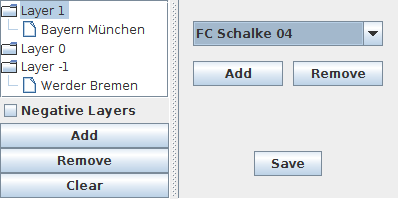
\includegraphics[width=\textwidth]{prefCreatorLayeredDialog.png}
	\caption{LayeredDialog}
	\label{img:prefCreatorLayeredDialog}
\end{figure}

Anschließend wird bei der Ausführung des Nodes, die Nodebaumstruktur des NodeDialogs durchlaufen.
Bei der Generierung des Preference Querys wird für jeden Prioritätsknoten ein 'PRIOR TO' und für jeden Paretoknoten ein 'AND' zum Query hinzugefügt. Bei der Erreichung einer Basispräferenz wird die für diese Präferenz entspreche Preference SQL Syntax hinzugefügt. Da die \enquote{CustomDimension} noch nicht von Preference SQL unterstützt wird, kommt es zu keinen Ergebnissen des Preference SQL Nodes, falls Preference Queries diese Präferenz enthalten. Andere Nodes, die mit den Scores arbeiten, können mit Präferenzen auf dieser Dimension umgehen. 

Falls beim Durchlaufen des Baumes für die Generierung des Score Querys eine Basispräferenz erreicht wird, wird die entsprechende Scoring Funktionen\footnote{Scoring Funktionen berechnen wie gut ein Datensatz einen Präferenz erfüllt. (siehe \cite{kiessling2002foundations})} der Präferenz in ein SQL Statemant konvertiert und dem Query hinzugefügt. Für die LOWEST Präferenz wird nur der Dimensionsname zur Query hinzugefügt. Das selbe gilt für die HIGHEST Präferenz, wofür hier jedoch noch mit $-1$ multipliziert wird. Dies ist sinnvoll, da dadurch für jede Basispräferenz die Datensätze mit den niedrigsten Scores gesucht werden können. Für jede AROUND Präferenz wird $abs(z-v)$, für jede BETWEEN Präferenz $v \in{[low, up]}$ then $0$ else if $v < low$ then $(low - v)$ else $(v - up)$ und für jede BOOLEAN Präferenz $-v$ als Statement zum Query hinzugefügt. In diesen Statements entspricht $v$ dem Dimensionsnamen, $z$ dem vom User eingegebenen Wert für die AROUND Präferenz und $low$ und $up$ für die entsprechenden Intervallgrenzen der BETWEEN Präferenz. 
Für die LAYERED Präferenz wird ein CASE Statement erstellt. Dieses gibt allen Datensätzen, die in der ausgewählten Dimension einen Wert in Layer 1 haben, einen Wert, der der Anzahl an positiven Layers  entspricht. Dieser Ausgabewert wird für jede weitere positive Layer reduziert. Für die erste negative Layer wird der Wert $-1$ vergeben und dieser für jede weitere Layer um $-1$ herunter gezählt. Alle Datensätze die einen Wert in Layer 0 haben, bekommen dementsprechend den Score 0. Zum Schluß wird das CASE Statement mit $-1$ multipliziert, damit auch diese Scores minimiert werden können.
In der Tabelle \ref{tbl:scoreComputation} wird dies an Beispielen genauer verdeutlicht. In der linken Spalte ist die Preference SQL Syntax der Präferenz zu sehen und in der rechten Spalte das entsprechende Score Query Statement. 

\begin{table}[H]
  \centering
  \begin{tabular}{|M{4cm}|M{10cm}|}
    \hline
    price LOWEST &  $price$ \\ \hline
    price HIGHEST & $-price$ \\ \hline
    price AROUND 16000 & $abs(16000-price)$ \\ \hline
    price BETWEEN 0,16000 & CASE WHEN price $\geq 0.0$ AND price $\leq 16000.0$ THEN $0$ WHEN price $< 0.0$ THEN ($0.0 - price$) WHEN $price > 16000.0$ THEN ($price-16000.0$) END \\ \hline
    price > 16000 BOOLEAN & price > 16000 \\ \hline
    color LAYERED (('green','black'), OTHERS, ('red')) & -(CASE WHEN color IN ('green', 'black') THEN 1 WHEN color IN ('brown', 'yellow', 'white', 'blue', 'silver') THEN 0 WHEN color IN ('red') THEN -1 END) \\ \hline
  \end{tabular}
  \newline\newline
  \caption{Beispielberechnung der Scores für Basispräferenzen}\label{tbl:scoreComputation}
\end{table}

Für den Präferenzbaum in Figur \ref{img:prefCreatorNodeDialog} werden folgende Queries erzeugt.

\textbf{Preference Query:}
\begin{verbatim}
SELECT * 
FROM (SELECT * FROM car) AS T 
PREFERRING ((price LOWEST PRIOR TO mileage LOWEST) 
AND horsepower HIGHEST)
\end{verbatim}

\textbf{Score Query:}
\begin{verbatim}
SELECT price AS column0,
mileage AS column1,
-(horsepower) AS column2 
FROM (SELECT * FROM car) as T
\end{verbatim}

Wie in den vorherigen Abschnitten erwähnt, müssen für die Berechnung einer Skyline Datensätze auf Dominanz getestet werden. Jedoch wird für diese Arbeit nicht mit den originalen Daten gearbeitet, sondern mit Scores. Diese repräsentieren wie gut ein Datensatz die Präferenzen des Users erfüllt. Für die Vergleiche zweier Datensätze wird neben den Scores zusätzlich die Baumstruktur des NodeDialogs benötigt. Damit diese an andere Nodes weitergegeben kann, muss sie in ein bestimmtes Format umgewandelt und als versteckte Eingabe weitergegeben werden. 
Für die Erstellung dieses Format wird wieder der Baum durchlaufen. Anfangs wird eine komplexe Präferenz $P_0$ erstellt, die dem Wurzelknoten des Baumes entspricht. Im Beispiel aus Abbildung \ref{img:prefCreatorNodeDialog} ist dies der Paretoknoten. Die Art\footnote{Die Art bezieht sich hierbei auf die Verknüpfungsart der Basispräferenzen. Somit sind nur die zwei Verknüpfungsarten 'Pareto' und 'Priority' möglich.} dieser Präferenz wird als erstes vermerkt. Als nächsten Schritt werden die Kinder dieses Knotens durchlaufen. Falls eines der Kinder ein Blatt und damit eine Basispräferenz ist, wird der entsprechende Spaltenname der Scoretabelle vermerkt. Falls es jedoch eine komplexe Präferenz (Prioritäts- oder Paretoknoten) ist, wird diese als nächste komplexe Präferenz vermerkt. Für den Beispielbaum ist einer der Kinder ein Prioritätsknoten und somit eine weitere komplexe Präferenz, die als $P_1$ vermerkt wird. Weiterhin hat der Paretoknoten noch die Basispräferenz horsepower LOWEST. Folglich wird der Spaltenname dieser Präferenz eingetragen. Nun wird dieser Vorgang für jede komplexe Präferenz in $P_0$ wiederholt. Da sowohl $P_0$ als auch $P_1$ keine weiteren komplexen Präferenzen besitzen, endet die Konvertierung des Baumes bei abgeschlossener Formatierung von $P_1$. Dieses Format wird als sogenannte Flowvariable an folgende Nodes weitergegeben. Flowvariablen besitzen einen Schlüssel mit dem der Inhalt abgerufen werden kann. Für die Formatierung der Präferenzbäume wird der Name der komplexen Präferenz als Schlüssel benutzt. Für den Beispielbaum aus Abbildung \ref{img:prefCreatorNodeDialog} ergeben sich somit die Flowvariablen in Tabelle \ref{tbl:serialization}.
Bei komplexen Präferenzen mit mehr als zwei Kinder, werden die Kinder in komplexe Präferenzen unterteilt. Für einen Baum mit einem einzelnen Paretoknoten, der drei Basispräferenzen als Kinder besitzt, ergeben sich die Flowvariablen in Tabelle \ref{tbl:threeChilds}.

\begin{table}[H]
  \centering
  \begin{tabular}{|M{4cm}|M{10cm}|}
    \hline 
    Flowvariblenschlüssel & Flowvaribleninhalt \\ \hline 
    P0 &  Pareto,P1,column2 \\ \hline
    P1 & Priority,column0,column1\\ \hline
  \end{tabular}
  \newline\newline
  \caption{Flowvariablen der serialisierten Baumstruktur}\label{tbl:serialization}
\end{table} 

\begin{table}[H]
  \centering
  \begin{tabular}{|M{4cm}|M{10cm}|}
    \hline   
    Flowvariblenschlüssel & Flowvaribleninhalt \\ \hline 
    P0 &  Pareto,P1,column2 \\ \hline
    P1 & Pareto,column0,column1\\ \hline
  \end{tabular}
  \newline\newline
  \caption{Die Flowvariablen für einen einzelnen Paretoknoten mit drei Basispräferenzen als Kinder}\label{tbl:threeChilds}
\end{table}

Nach Ausführung des Nodes liegt das in den Node eingehende DatabasePortObject, der optionale BufferedDataTable mit den Scores und die Flowvariablen, die den Score Query, Preference Query und die formatierte  Baumstruktur enthalten, vor.
Mit diesen Daten kann nun die Skyline berechnet werden.
%% ==============================
\section{Preference SQL Extract Node}
\label{ch:Implementierung:sec:prefSQLExtract}
%% ==============================
Dieser Abschnitt befasst sich mit dem Preference SQL Extract Node (siehe Abbildung \ref{img:prefSQLExtractorLogo}). Dieser nimmt als Eingabe ein DatabasePortObject, welches von einem Preference Creator Node kommen muss. Dies hat den Grund das mit dem DatabasePortObject des Preference Creator Nodes auch versteckte Flowvariablen in den Node kommen, die den benötigten Preference Query beinhalten.

\begin{figure}[H]
	\centering
	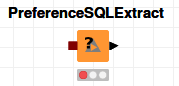
\includegraphics{prefSQLExtractorLogo.png}
	\caption{Preference SQL Extract Node}
	\label{img:prefSQLExtractorLogo}
\end{figure}

Im NodeModel wird ein leerer BufferedDataTable mit einer Spalte und einer Reihe erstellt. Dieser einen Zelle wird der Preference Query hinzugefügt. Der User kann nach erfolgreicher Ausführung des Nodes diesen BufferedDataTable öffnen und den entsprechenden Query kopieren.
%% ==============================
\section{Preference SQL Node}
\label{ch:Implementierung:sec:prefSQL}
%% ==============================
\begin{figure}[H]
	\centering
	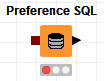
\includegraphics{prefSqlLogo.png}
	\caption{Preference SQL Node}
	\label{img:prefSQLLogo}
\end{figure}

Der Preference SQL Node benötigt als Eingabe ein DatabasePortObject. Da der Preference Query benötigt wird, erscheint eine Fehlermeldung, falls dieser nicht vorhanden ist. Infolgedessen sind nur DatabasePortObjects von einem Preference Creator Node zulässig.

Bisher ist für diesen Node die Abfrage des Preference Query nur auf der PostgreSQL Datenbank des gemini Servers der Universität Augsburg möglich. Jedoch soll in der Zukunft diese Abfrage auf diesen Server weitergeleitet werden, damit auch Abfragen von anderen Datenbanken ermöglicht werden.
Derzeit fragt der Node mit der vorhandenen Datenbankverbindung den Preference Query ab und liefert die entsprechenden Daten als BufferedDataTable zurück. Die Datentabelle kann vom Benutzer nach Ausführung des Nodes betrachtet werden und nach seinen Wünschen sortiert werden. Die Datentabelle enthält die Datensätze, die die im Preference Creator Node erstellten Präferenzen am besten erfüllen. Somit entspricht diese Ausgabe einer Skyline basierend auf den vom User erstellten Präferenzen.
%% ==============================
\section{Block Nested Loop Node}
\label{ch:Implementierung:sec:bnlNode}
%% ==============================
\begin{figure}[H]
	\centering
	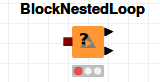
\includegraphics{bnlLogo.png}
	\caption{Block Nested Loop Node}
	\label{img:bnlLogo}
\end{figure}

Der Block Nested Loop Node benötigt als Eingabe nur ein DatabasePortObject. Es wird geprüft, ob ein Score Query und die formatierte Baumstruktur vorhanden sind. Falls dies nicht der Fall ist, wird ein Fehler an den User ausgegeben.
Durch die Abfrage des Score Query an die Datenbankverbindung kann die Scoretabelle erzeugt werden.

Mithilfe der Scores und dem Block Nested Loop Algorithmus kann die Skyline berechnet werden.
Hierfür wird zuerst der Block Nested Loop Algorithmus standardmäßig nach Kapitel \ref{ch:Analyse:sec:skyAlgos:subsec:bnl} ausgeführt. Falls die Dominanz zwischen zwei Datensätzen geprüft werden muss, wird zuerst die konvertierte Baumstruktur, welche komplexe Präferenzen enthält, durchlaufen.
Wie in Abschnitt \ref{ch:Implementierung:sec:prefCreatorNode} erwähnt, sieht die Struktur von komplexen Präferenzen folgendermaßen aus: Art der Präferenzverknüpfung, Präferenz 1, Präferenz 2 (siehe Tabelle \ref{tbl:serialization}).
Dabei können Präferenz 1 und 2 weitere komplexe Präferenzen sein, die auch durchlaufen werden müssen bis eine komplexe Präferenz gefunden wird, die nur aus Basispräferenzen bzw. den entsprechenden Spaltennamen der Scoretabelle besteht.
Das Durchlaufen wird rekursiv durchgeführt und startet mit einer der folgenden Funktionen. Die erste komplexe Präferenz $P0$ und deren Art von Präferenzverknüpfung bestimmen mit welcher Formel gestartet wird.
Präferenzverknüpfungen können vom Typ 'Priority' oder 'Pareto' sein.

Gegeben seien zwei Datensätze $D_1$ und $D_2$ und zwei Präferenzen $P_1$ und $P_2$.
Es soll geprüft werden, dass Datensatz $D_1$ $D_2$ dominiert: $D_1 <_P D_2$, wobei $P$ eine Verknüpfung der beiden Präferenzen $P_1$ und $P_2$ darstellt.

Die Prüfung der Dominanz hängt von der Art der Präferenzverknüpfung ab. Für die Prioritätsverknüpfung werden folgende Formeln benutzt:

\textbf{Definition Priorisierung:} \\
Für die Präferenzen $P_1$ und $P_2$ wird die Priorisierung wie folgt definiert: $P = P_1$ \& $P_2:$

Dominanz Formel: \\
$D_1 <_P D_2$ gdw. $D_1 <_{P_1} D_2 \lor (D_1 =_{P_1} D_2 \land D_1 <_{P_2} D_2)$ \\ \\
Äquivalenz Formel: \\
$D_1 =_P D_2$ gdw. $D_1 =_{P_1} D_2 \land D_1 =_{P_2} D_2$ \\

Falls jedoch die Art der Verknüpfung vom Typ Pareto vorliegt, wird die Dominanz mit folgenden Formeln geprüft:

\textbf{Definition Pareto:} \\
Für Präferenzen $P_1$ und $P_2$ wird die Paretoverknüpfung wie folgt definiert: $P = P_1 \otimes P_2:$ \\ \\
Dominanz Formel:\\
$D_1  <_P D_2$ gdw. $(D_1 <_{P_1} D_2 \land (D_1 <_{P_2} D_2 \lor D_1 =_{P_2} D_2)) \lor (D_1 <_{P_2} D_2 \land (D_1 <_{P_1} D_2 \lor D_1 =_{P_1} D_2))$ \\ \\
Äquivalenz Formel: \\
$D_1 =_P D_2$ gdw. $D_1 =_{P_1} D_2 \land D_1 =_{P_2} D_2$ \\

Wie schon im Abschnitt \ref{ch:Implementierung:sec:prefCreatorNode} erwähnt, werden die Scores so bestimmt, dass alle einheitlich minimiert werden können. Dadurch besteht die Skyline meistens nur aus Datensätzen mit niedrigen Scores. Falls einer der beiden Präferenzen, $P_1$ oder $P_2$, eine Basispräferenz ist, werden die Scores für diese Präferenz von beiden Datensätzen verglichen. Falls jedoch $P_1$ oder $P_2$ weitere komplexen Präferenzen sind, müssen zuerst weitere Formeln berechnet werden. Diese Vorgehensweise wird nun anhand eines Beispiels veranschaulicht.

\begin{table}[H]
  \centering
  \begin{tabular}{|M{3cm}|M{2.5cm}|M{2.5cm}|M{2.5cm}|}
    \hline 
    Datensatz & column0 & column1 & column2 \\ \hline 
    Datensatz 1 & 30 & 12 & 4\\ \hline
    Datensatz 2 & 30 & 15 & 2\\ \hline
  \end{tabular}
  \newline\newline
  \caption{Beispielscores}
  \label{tbl:scoresExample}
\end{table} 


Es wird angenommen, dass die formatierte Nodebaumstruktur aus Tabelle \ref{tbl:serialization} und die Scores aus Tabelle \ref{tbl:scoresExample} vorliegen. Die Dominanz zwischen den beiden Datensätzen wird geprüft, indem die entsprechende Dominanz Formel von $P_0$ verwendet wird. Da $P_0$ eine Paretoverknüpfung ist, wird die Dominanzformel für Paretoverknüpfungen angewandt. 
Jedoch besitzt $P_0$ eine komplexe Präferenz $P_1$, wodurch die Werte für $D_1 <_{P_1} D_2$ und $D_1 =_{P_1} D_2$ zuerst durch entsprechende Formeln bestimmt werden müssen. Für $D_1 <_{P_1} D_2$ wird die Dominanz Formel für Priorisierungen und für $D_1 =_{P_1} D_2$ die entsprechende Äquivalenz Formel benutzt. Für $P_1$ werden die jeweiligen Scores miteinander verglichen, da $P_1$ zwei Basispräferenzen verknüpft. 

$D_1 <_{P_1} D_2: 30 < 30 \lor (30==30 \land 12 < 15)$ \\
$D_1 =_{P_1} D_2: 30 == 30 \land 12 == 15$ 

Der erste Ausdruck ergibt $true$ zurück, wohingegen der zweite Ausdruck $false$ zurück gibt. Diese Werte können nun in die Dominanz Formel für $P_0$ eingesetzt werden.

$D_1 <_{P_0} D_2: (true \land (4 < 2 \lor 4==2)) \lor (4 < 2 \land (true \lor false))$ \\ 

Somit ergibt sich, dass die beiden Datensätze sich nicht dominieren, da $D_1 <_{P_0} D_2$ $false$ zurück gibt.

Der Block-Nested-Loop Algorithmus läuft ganz normal durch bis alle undominierten Datensätze der Scoretabelle gefunden sind. Der Node kann dann anhand der RowIDs dieser undominierten Datensätze die undominierten Datensätze der Originaltabelle ausgeben, da diese die gleichen RowIDs besitzen.

Der NodeDialog erlaubt es dem Benutzer für den Block-Nested-Loop Algorithmus eine Größe für das Fenster $w$ zu bestimmen. Weitere Eingaben für diesen Node sind nicht nötig, da die meisten Einstellungen durch Flowvariablen des PreferenceCreator Nodes schon vorhanden sind.

Der Block-Nested-Loop ermöglicht auch eine Darstellung der Datensätze mittels eines NodeViews. In Abbildung \ref{img:bnlSkyline} kann eine Skyline des Autodatensatzes für die Präferenzen in Figur \ref{img:prefCreatorNodeDialog} betrachtet werden.

\begin{figure}[H]
	\centering
	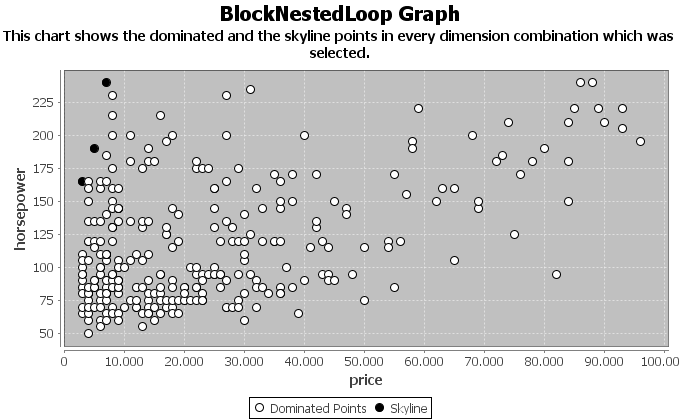
\includegraphics[width=\textwidth]{bnlSkyline.png}
	\caption{Skyline-Datensätze, die durch die Block-Nested-Loop Node entsteht}
	\label{img:bnlSkyline}
\end{figure}
%% ==============================
\section{Domination Maximizer Node}
\label{ch:Implementierung:sec:dominationMaximizerNode}
%% ==============================
\begin{figure}[H]
	\centering
	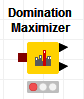
\includegraphics{domMaximizerLogo.png}
	\caption{Domination Maximizer Node}
	\label{img:domMaximierLogo}
\end{figure}

Der DominationMaximizer Node berechnet die repräsentative Skyline basierend auf den Originaldaten und benötigt daher keine Skyline. Die Eingabe ist wieder ein DatabasePortObject eines Preference Creator Nodes.

Der im NodeModel auszuführende Algorithmus für diesen Node wurde in Kapitel \ref{ch:Analyse:sec:repSkyAlgos:subsec:domMax} vorgestellt. Die Dominanz wird identisch zum Block Nested Loop Node durch die Nodebaumstruktur und den entsprechenden Formeln berechnet.

Die erste Ausgabe besteht aus den $k$ Skylinedatensätzen, bei der die Anzahl der dominierten Datensätze maximal ist. Die zweite Ausgabe ist die Skyline $S_P$, die während der Durchführung des Algorithmus berechnet wird. Mit diesen beiden Ausgaben kann mithilfe des Nodes in Abschnitt \ref{ch:Implementierung:sec:skyVisualizer} ein Graph erstellt werden. 

Der NodeDialog erlaubt es dem User die Größe der repräsentativen Skyline festzulegen. Für eine schnelle Ausführung des Nodes wird wie bei jedem anderen Node für die Eingabeparameter ein Standardwert festgelegt. Somit kann der User den Node nach Erstellung ausführen ohne jemals den NodeDialog geöffnet zu haben.   
%% ==============================
\section{Distance Based Resolver Node}
\label{ch:Implementierung:sec:distBasedResolverNode}
%% ==============================
\begin{figure}[H]
	\centering
	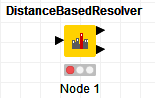
\includegraphics{distBasedResolverLogo.png}
	\caption{Distance Based Resolver Node}
	\label{img:distBasedResolverLogo}
\end{figure}

Der Distance BasedResolver Node benötigt als Eingabe zwei BufferedDataTables, die nur Datensätze besitzen, die sich basierend auf den Präferenzen nicht gegenseitig dominieren. Die erste Datentabelle entspricht der Skyline der Originaldaten, wohingegen die zweite Datentabelle die Skyline der Scores ist.

Der Algorithmus dieses Nodes ist in Kapitel \ref{ch:Analyse:sec:repSkyAlgos:subsec:disBasedRepSky} zu finden. Wie zu erkennen ist, beruht die Berechnung der Distanz nur auf zwei Dimensionen. Aus diesem Grund gibt der Node bei mehr als drei Dimensionen dem User eine Warnung aus, dass für die Berechnung der repräsentativen Skyline nur die ersten zwei Dimensionen betrachtet werden.

Die erste Ausgabe entspricht der repräsentativen Skyline und enthält somit alle Datensätze, die vom Algorithmus zurückgegeben werden. Die zweite Ausgabe ist die Skyline der Originaldaten und dient mit der repräsentativen Skyline als Eingabe für den Node in Kapitel \ref{ch:Implementierung:sec:skyVisualizer}.

Der NodeDialog bietet dem User ein Eingabefenster, um die Anzahl der repräsentativen Skylinedatensätze zu bestimmen. Falls diese Zahl höher oder gleich der Anzahl der Datensätze der Eingabe ist, werden alle Datensätze ohne Berechnung des Algorithmus ausgegeben.
%% ==============================
\section{Diversity Significance Based Resolver Node}
\label{ch:Implementierung:sec:eGreedyNode}
%% ==============================
\begin{figure}[H]
	\centering
	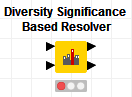
\includegraphics{eGreedyLogo.png}
	\caption{Diversity Significance Based Resolver}
	\label{img:eGreedyLogo}
\end{figure}

Dieser Node implementiert den Algorithmus aus Kapitel \ref{ch:Analyse:sec:repSkyAlgos:subsec:eGreedy} und benötigt daher als Eingabe eine Skyline. Aus dieser werden aufgrund von Diversität und Signifikanz die $k$ besten Datensätzen ausgegeben.

Die Anzahl der repräsentativen Skyline Datensätze, die ausgegeben werden sollen, kann der Benutzer im NodeDialog einstellen. Zusätzlich besteht die Möglichkeit dort Diversitäts- und Signifikanzfaktor einzustellen. Der Diversitätsfaktor steht für $\lambda$ und der Signifikanzfaktor für $1-\lambda$. Bei Eingabe einer dieser Parameter, wird der andere dementsprechend angepasst, sodass die Summe beider Werte immer $1$ ergibt.
Für die Berechnung der Signifikanz wird eine Sigmoidfunktion benutzt, da diese Thresholds des Benutzers berücksichtigen kann. Somit kann der User im NodeDialog für jede Dimension entscheiden, ob er einen einzelnen Threshold, einen Intervallthreshold oder gar keinen eingeben möchte. \footnote{siehe Figur \ref{img:eGreedyNodeDialog}} Falls der User vor der Ausführung des Nodes niemals den NodeDialog geöffnet und keine Thresholds angegeben hat, werden alle Datensätze als gleich signifikant angesehen und somit wird nur die Diversität berücksichtigt. 

\begin{figure}[H]
	\centering
	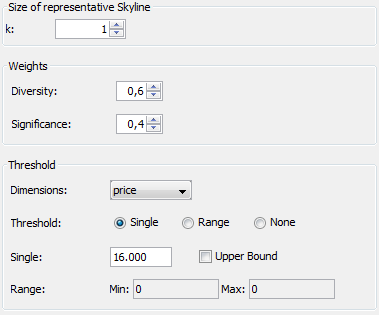
\includegraphics{eGreedyNodeDialog.png}
	\caption{NodeDialog des E-Greedy Nodes}
	\label{img:eGreedyNodeDialog}
\end{figure}

Nach Ausführung des Algorithmus werden zwei Outputs ausgegeben. Die $k$ repräsentativen Skylinedatensätze und die ursprüngliche Skyline. Für die Skyline aus Figur \ref{img:bnlSkyline} und der Eingaben im NodeDialog ergibt sich die repräsentative Skyline, die in Abbildung \ref{img:eGreedyOutput} zu sehen ist.

\begin{figure}[H]
	\centering
	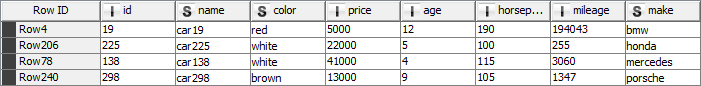
\includegraphics[width=\textwidth]{eGreedyOutput.png}
	\caption{Repräsentative Skyline, die durch den E-Greedy Node entsteht}
	\label{img:eGreedyOut}
\end{figure}
%% ==============================
\section{(Representative) Skyline Visualizer Node}
\label{ch:Implementierung:sec:skyVisualizer}
%% ==============================
\begin{figure}[H]
	\centering
	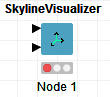
\includegraphics{skyVisualizerLogo.png}
	\caption{(Representative) Skyline Visualizer Node}
	\label{img:skyVisualizerLogo}
\end{figure}

Der (Representative) Skyline Visualizer Node benötigt zwei BufferedDataTables als Eingabe. Die Daten beider Tabellen werden in einem Koordinatensystem, dem NodeView des Nodes, angezeigt. Dafür werden alle Dimensionen bestimmt, die Präferenzen besitzen und numerisch sind. Der View wird nur bei Betrachtung von zwei oder drei Dimensionen erstellt. Für drei Dimensionen wird ein Koordinatensystem für jede Dimensionskombination erstellt.

Im NodeDialog (siehe \ref{img:skyVisualizerNodeDialog}) kann der User einstellen wie er seinen Graph beschriftet haben möchte. Zur Auswahl stehen die Beschriftung für einen repräsentativen Skyline Graphen (weiße Punkte: Skyline, schwarz: representative Skyline) oder einen Skyline Graphen (weiß: Dominated Points Punkte, schwarz: Skyline). Falls dem User keiner dieser Einstellungen gefällt, kann er die Überschrift und die Beschreibung des Graphen auch selbst in den Eingabefeldern des NodeDialogs eintragen. Zusätzlich zu diesen Einstellungen kann der Benutzer die Dimensionen für die Erstellung des Views auswählen. Somit ist auch eine Generierung des Views bei mehr als vier vorhandenen Dimensionen möglich.

\begin{figure}[H]
	\centering
	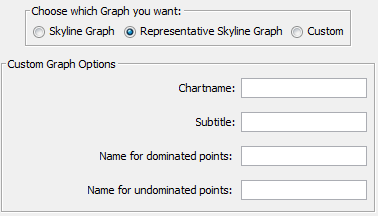
\includegraphics{skyVisualizerNodeDialog.png}
	\caption{NodeDialog des SkylineVisualizer Nodes}
	\label{img:skyVisualizerNodeDialog}
\end{figure}

Bei einer Betrachtung von drei Dimensionen wird ein View wie in Abbildung \ref{img:skyVisiualizerView2} erstellt. Bei Betrachtung von nur zwei Dimensionen, entsteht ein View wie in Abbildung \ref{img:skyVisiualizerView1}.

\begin{figure}[H]
	\centering
	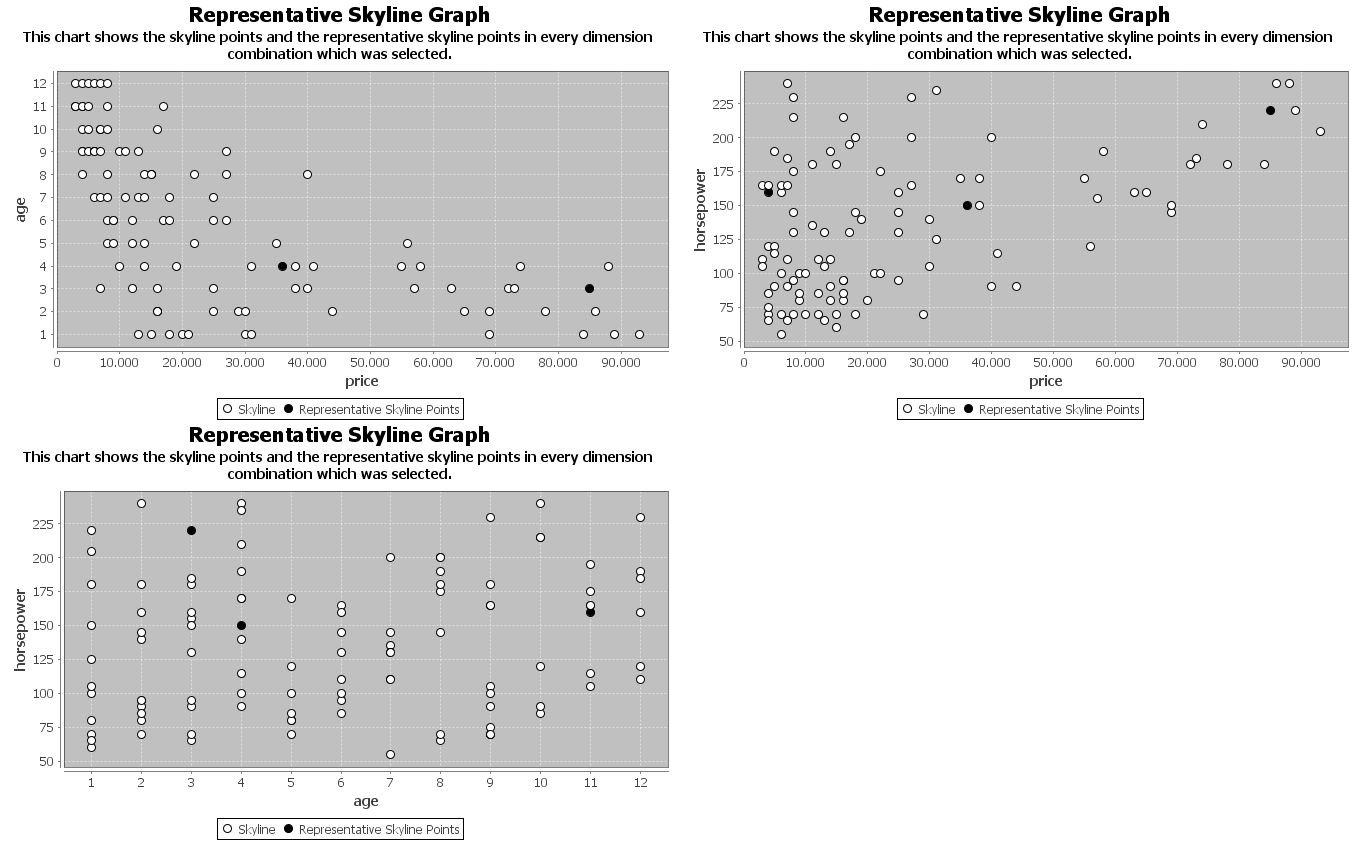
\includegraphics[width=\textwidth]{skyVisualizerView2.png}
	\caption{View des (Representative) Skyline Visualizer Nodes für drei Dimensionen}
	\label{img:skyVisiualizerView2}
\end{figure}

\begin{figure}[H]
	\centering
	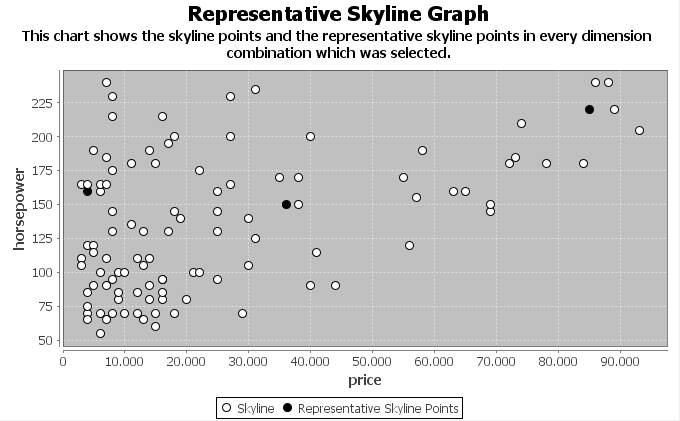
\includegraphics[width=\textwidth]{skyVisualizerView1.png}
	\caption{View des (Representative) Skyline Visualizer Nodes für zwei Dimensionen}
	\label{img:skyVisiualizerView1}
\end{figure}
%% ==============================
%%% End: 